\chapter{Lattice dynamics in LSCO+O: A study using ToF and ab-initio MD}

\section{Introduction}
We are performing inelastic neutron time-of-flight experiments on a series of La$_{2-x}$Sr$_{x}$CuO$_{4+\delta}$ powdered samples in order to better understand the curious relationship between mobile (O) and static (Sr) dopants. By careful analysis of the changes in the phonon spectra, we hope to better understand the role of mobile dopants and their relationship to superconductivity.

\section{Samples}
Experiments were performed on 4 powdered samples of roughly 5 grams each: LCO (no $T_\text{c}$), LSCO (no $T_\text{c}$), LCO+O ($T_\text{c} = \SI{40}{\kelvin}$), LSCO3+O ($T_\text{c} = \SI{40}{\kelvin}$). Powders were synthesized by mixing \ce{La2O3}, \ce{CuO} and (in the case of Sr doping) \ce{SrCO3} followed by calcination in a box furnace at 950$^\circ \, \text{C}$ for 48 hours. Intercalation of oxygen was performed by electrochemical methods at University of Copenhagen. This method has previously been described elsewhere\cite{Blakeslee1998}.

\section{Experimental}
Experiments were performed at the thermal neutron time-of-flight spectrometer IN4c at Institut Laue-Langevin in Grenoble, France. In order to see excitations in the \SIrange{5}{100}{\milli\eV} range, each sample/temperature was measured at three different incident neutron wavelengths as shown in Table \ref{tab:in4}. Sample was mounted in a cadmium frame as shown in Figure \ref{fig:sample_sqw}B. Each of the 4 samples was measured for 3.5-4 hours per temperature/wavelength combination. 

\begin{figure}
    \centering
    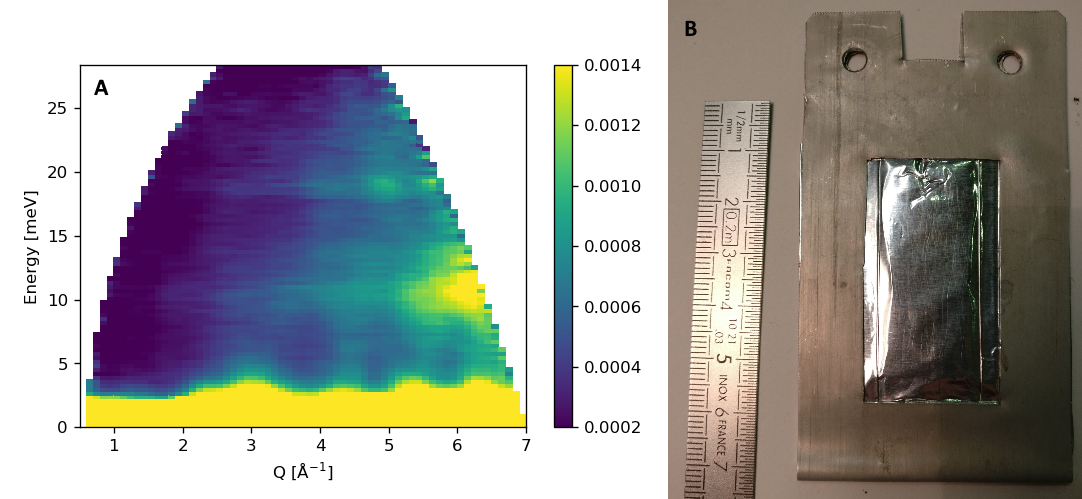
\includegraphics[width=\textwidth]{fig/gdos/sample_sqw.png}
    \caption[$S(\bm{q}, \omega)$ map and picture of sample]{\textbf{A}: $S(\bm{q}, \omega)$ map of LSCO at \SI{10}{K} with \SI{1.6}{\angstrom} incident energy. Data has normalized by the Bose factor. \textbf{B:} Sample mounted in cadmium frame.}
    \label{fig:sample_sqw}
\end{figure}

\begin{table}[b]
    \centering
    \begin{tabular}{lllll}\toprule
    $\lambda$ [\AA] & Monochromator  & $k$ [\AA$^{-1}$] & E [meV] & Sapphire Filter     \\ \midrule
    1.6             & PG004 & 3.93            & 31.95   & \texttt{IN}  \\
    1.1             & PG004 & 5.71            & 67.61   & \texttt{IN}  \\
    0.85            & Cu220 & 7.39            & 113.22  & \texttt{OUT} \\ \bottomrule
    \end{tabular}
    \caption[IN4: Incident energies]{Overview of incident energies used in the experiments.}
    \label{tab:in4}
\end{table}

The raw time-of-flight data was reduced to $S(\bm{q},\omega)$ using the \texttt{Mantid} \cite{Arnold2014} software. Background was corrected using a Vanadium scan. Due to the isotropic nature of the powder, we only consider the magnitude of $\bm{q}$ and the resulting data can be viewed in two dimensions as shown in Figure \ref{fig:sample_sqw}A. Obtaining the density-of-states is done in Mantid with the \texttt{ComputeIncoherentDOS} algorithm, using the following expression for the 1-phonon incoherent scattering function:

 \[ S^{(1)}_{\mathrm{inc}}(Q,E) = \exp\left(-2\bar{W}(Q)\right) \frac{Q^2}{E} \langle n+\frac{1}{2}\pm\frac{1}{2} \rangle \left[ \sum_k \frac{\sigma_k^{\mathrm{scatt}}}{2m_k} g_k(E) \right]\, , \]
 
 \noindent where $\bar{W} = Q^2 \langle u \rangle / 2$ with $\langle u \rangle$ being the average mean-squared displacement. As we have no information about $\langle u \rangle$, it is set to 0 in the following calculations. $n$ is the Bose factor and $E$ is the energy transfer. Finally, the term in brackets is the neutron-weighted density of states with $k$ running over the different elements in our sample. The calculated DOS is given in milibarns/steredians per formula unit per meV. It is not possible to obtain DOS in states per meV as this requires a pure element.
 
 In order to get meaningful results from this procedure, some further reduction of the data is usually required. Generally, one chooses a range of $Q$ and $E$ to sum over along with a re-binning of $E$. Since the measured ranges are different between incident energies, these ranges are chosen for each of the three configurations (see Table \ref{tab:in4}). The parameters used for our calculations are shown in Table \ref{tab:qeranges}.
 
\begin{table}[b]
 \centering
\begin{tabular}{llllll}
\toprule
$\lambda$ [\AA] & $Q_\text{min}$ [\AA$^{-1}$] & $Q_\text{max}$ [\AA$^{-1}$] & $E_\text{min}$ [meV] & $E_\text{max}$ [meV] & $\Delta E$ [meV] \\ \midrule
1.6             & 2.0                         & 6.0                         & 4.0                  & 20.0                 & 0.2              \\
1.1             & 2.5                         & 7.5                         & 7.0                  & 45.0                 & 0.4              \\
0.85            & 5.0                         & 9.0                         & 20.0                 & 95.0                 & 1.0              \\ \bottomrule
\end{tabular}
 \caption[IN4: $Q$ and $E$ windows for DOS integration]{$Q$ and $E$-ranges used in the computation of DOS.}
 \label{tab:qeranges}
\end{table}

\begin{figure}
    \centering
    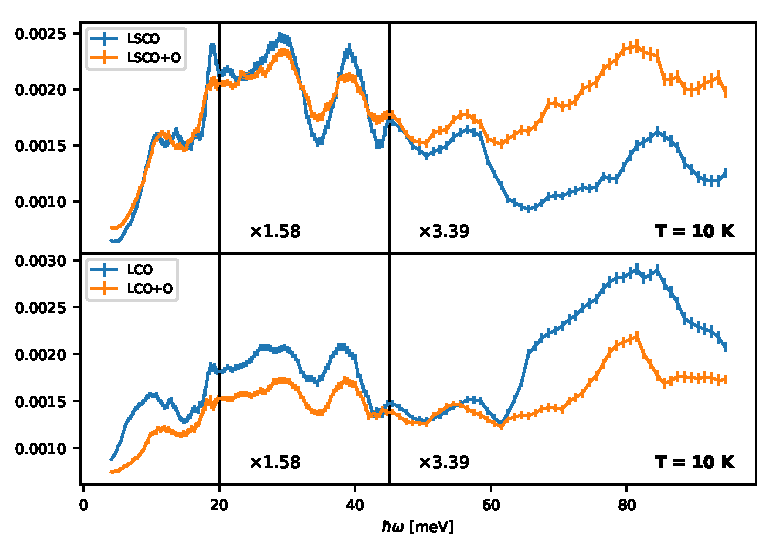
\includegraphics[width=\textwidth]{fig/gdos/gdos_10K.pdf}
    \caption[gDOS at \SI{10}{\kelvin}]{GDOS at \SI{10}{\kelvin}}
    \label{fig:gdos_10k}
\end{figure}

\begin{figure}
    \centering
    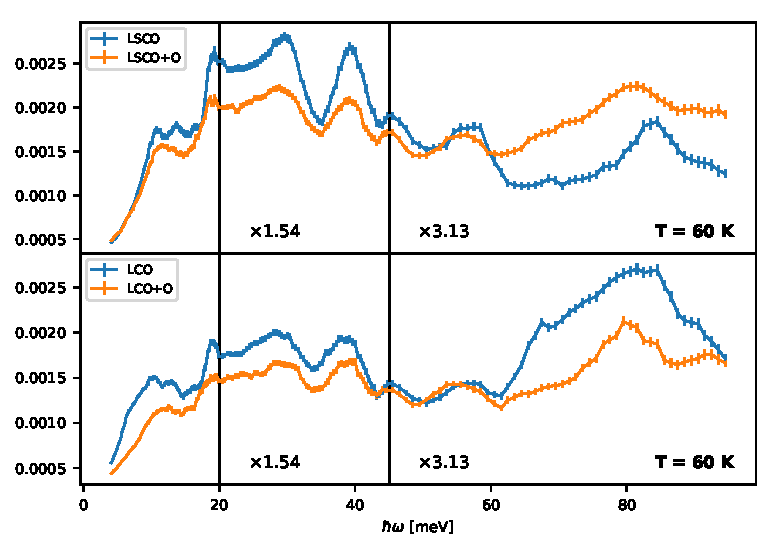
\includegraphics[width=\textwidth]{fig/gdos/gdos_60K.pdf}
    \caption[gDOS at \SI{60}{\kelvin}]{GDOS at \SI{60}{\kelvin}}
    \label{fig:gdos_60k}
\end{figure}

\begin{figure}
    \centering
    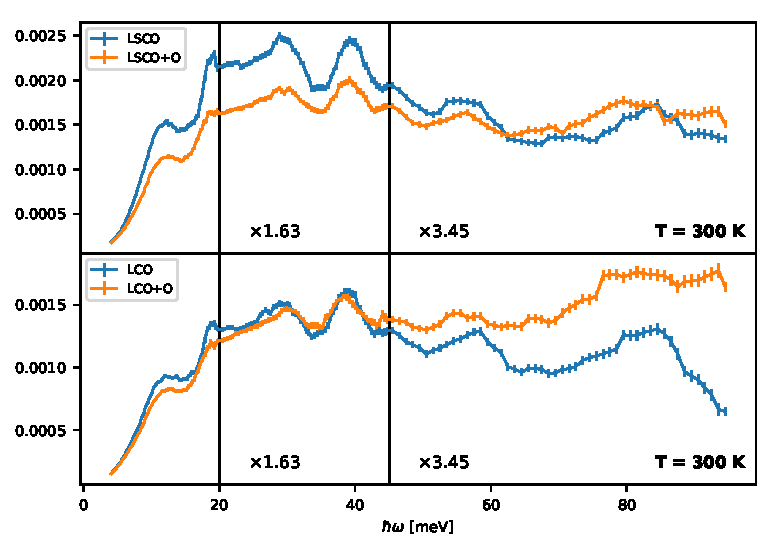
\includegraphics[width=\textwidth]{fig/gdos/gdos_300K.pdf}
    \caption[gDOS at \SI{300}{\kelvin}]{GDOS at \SI{300}{\kelvin}}
    \label{fig:gdos_300k}
\end{figure}